\documentclass[journel,12pt,twocoloums]{IEEEtran}

\title{Assignment 4-Probability and Random Variable}
\author{Annu-EE21RESCH01010}
\date{13 January 2020}

\usepackage{amsthm}
\usepackage{graphicx}
\usepackage{mathrsfs}
\usepackage{txfonts}
\usepackage{stfloats}
\usepackage{pgfplots}
\usepackage{cite}
\usepackage{cases}
\usepackage{mathtools}
\usepackage{caption}
\usepackage{enumerate}	
\usepackage{enumitem}
\usepackage{amsmath}
\usepackage[utf8]{inputenc}
\usepackage[english]{babel}
\usepackage{multicol}
%\usepackage{xtab}
\usepackage{longtable}
\usepackage{multirow}
%\usepackage{algorithm}
%\usepackage{algpseudocode}
\usepackage{enumitem}
\usepackage{mathtools}
\usepackage{gensymb}
\usepackage{hyperref}
%\usepackage[framemethod=tikz]{mdframed}
\usepackage{listings}
    %\usepackage[latin1]{inputenc}                                 %%
    \usepackage{color}                                            %%
    \usepackage{array}                                            %%
    \usepackage{longtable}                                        %%
    \usepackage{calc}                                             %%
    \usepackage{multirow}                                         %%
    \usepackage{hhline}                                           %%
    \usepackage{ifthen}                                         %%
  \providecommand{\nCr}[2]{\,^{#1}C_{#2}}
  \providecommand{\nPr}[2]{\,^{#1}P_{#2}}
  \lstset{
%language=C,
frame=single, 
breaklines=true,
columns=fullflexible
}

 \begin{document}
 \maketitle
\textbf{Download latex code from here-}\\
\begin{lstlisting}
 https://github.com/annu100/AI5002-Probability-and-Random-variables/tree/main/ASSIGNMENT_4
 \end{lstlisting}
 \section{Problem Statement-Problem 3.10}
How many times must a man toss a fair coin
so that the probability of having at least one
head is more than 90%?
\section{Solutions}

Let r be the number for getting no. of  heads. \\
let n =total no. of times a coin is tossed\\
therefore, q=1-p ,which is probability of getting a tail.Since it is the case of fair coin, therefore p=0.5 and q =0.5\\
\begin{align}
    p=\frac{1}{2} \\
    q=1-\frac{1}{2}=\frac{1}{2}
\end{align}
From bernaulli's distribution, we know\\
\begin{align}
    Pr(X=r)= \nCr{n}{r} p^r q^{n-r}  \\
    X \sim Bin(n,p=0.5)
\end{align}
We are required to find the number of trials such that the sample  probability of having at least one
head is more than 90%\\
\begin{align}
    Pr(X \ge 1) &=1-Pr(X=0)\\
                &=1-\nCr{n}{0} 0.5^0 0.5^{n-0} >0.9 \\
                &=1-(\frac{1}{2})^n >0.9\\
                &=(\frac{1}{2})^n < 0.1\\
                &= 2^{n} >10
\end{align}
This implies $n \ge 4$


Therefore, the required number of trials must be greater than or equal to 4.From graph,we can also see\\

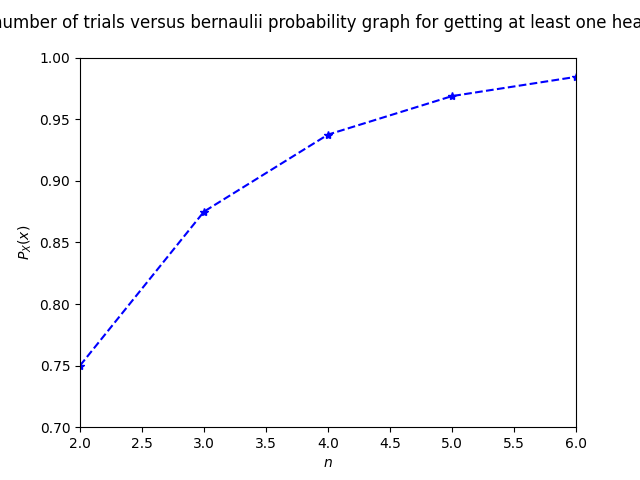
\includegraphics[width=\coloumnwidth]{Figure_1.png}
\textbf{Above is is the graph of no. of trails versus probability }
            
\end{document}
        

